\section{Background}
\label{sec:background}

\subsection{Traditional Approaches Towards RAG}
Retrieval augmented generation (RAG) aims to address hallucinations and factual inaccuracies in LLM-generated content. RAG infuses 
external knowledge~\cite{peng2023check, lazaridou2022internet}, such as knowledge bases and web documents, while prompting LLMs to help generate responses grounded on relevant information. The integration of RAG-based workflows in prompting LLMs has enjoyed widespread adoption, enhancing the suitability of LLMs for real-world applications. Development of a RAG system often begins with an indexing step, which involves cleaning and segmenting the documents --- segmentation is required to prepare chunks of information that carry meaningful and strong signals, and in addition, to fit into an LLM's context window (when using LLMs with limited context windows). Each chunk is then encoded into a vector representation using an embedding model and stored in a vector database. This step is essential for enabling efficient similarity searches in the subsequent retrieval phase. As shown in Figure~\ref{fig:sys-rag2}, the following are the standard phases of a traditional RAG workflow:

\stitle{Retrieval.} Given a user query, a RAG system employs an encoding model used during indexing to transform the query into a vector representation and calculates the similarity scores between two vectors: query and candidate text chunks within the indexed corpus. Based on these scores, the system retrieves the top-$K$ chunks with the highest similarity to the query, which are then used as the expanded context for the next stage.

\stitle{Augmentation.} The selected chunks are incorporated into a prompt as expanded context to provide additional relevant information. The goal of such enhancement is to reduce hallucination and improve accuracy of the model’s response. By providing targeted context, the RAG system ensures the model can ground its answer in the most pertinent retrieved data.

\stitle{Generation.} The user query, along with the augmented context of selected documents, is synthesized into a coherent prompt, which is then provided to an LLM that will perform the final generation task. Depending on the task requirements, the model may either draw upon its internal knowledge or limit its response to information in the provided documents. 

\subsection{Limitations of RAGs}

Traditional approaches to RAG do not directly apply to real-world scenarios due to the heterogeneity of data, the complexity of workflows, and the strict constraints on expected task performances.

\subsubsection{Lack of Robust Deliberation}

\newcommand{\crimson}{red}
\newcommand{\darkgreen}{green}

\begin{table*}[!htb]
    \centering
    \scriptsize
    % \resizebox{\textwidth}{!}{
    \begin{tabular}{p{15.5cm}}
        \toprule
        \textbf{Triple: }(Chicago, country, United States of America) \hfill \textbf{Entity Popularity: $95.0\%ile$}\\
        \textbf{Question:} What country is Chicago located in? \hfill\textbf{Entity-Relation Popularity: $97.4\%ile$}\\ %  Popular + no retrieval error\\
        \textbf{LM Answer:} United States {\color{\darkgreen}[Correct]}\\
        \textbf{Context: } The Chicago Municipal Tuberculosis Sanitarium was located in Chicago, Illinois, USA.\dots{\color{\darkgreen}[Correct Retrieval]}\\
        \textbf{RALM Answer:} USA {\color{\darkgreen}[Correct]}\\\midrule
        \textbf{Triple: }(George H.W. Bush, educated at, Yale University) \hfill \textbf{Entity Popularity: $89.5\%ile$}\\
        \textbf{Question:} What educational institution did George H.W. Bush attend? \hfill \textbf{Entity-Relation Popularity: $41.8\%ile$}\\% Popular + retrieval error\\
        \textbf{LM Answer:} Yale University {\color{\darkgreen}[Correct]}\\
        \textbf{Context: } The George H.W. Bush Presidential Library is located on a site on the west campus of Texas A\&M University in College Station, Texas.\dots {\color{\crimson}[Wrong Retrieval]}\\
        \textbf{RALM Answer:} Texas A\&M University {\color{\crimson}[Wrong]}\\\midrule
        \textbf{Triple: }(Ellen Litman, educated at, University of Pittsburgh) \hfill \textbf{Entity Popularity: $10.3\%ile$}\\
        \textbf{Question:} What educational institution was Ellen Litman educated at? \hfill \textbf{Entity-Relation Popularity: $17.9\%ile$} \\ % Less Popular + no retrieval error\\
        \textbf{LM Answer:} Stanford University {\color{\crimson}[Wrong]} \\
        \textbf{Context: } Ellen Litman Ellen Litman (born 1973) is an American novelist. She received the Rona Jaffe Foundation Writers' Award in 2006. Born in Moscow, Russia, she emigrated with her parents in 1992 to Pittsburgh, Pennsylvania. She was educated at the University of Pittsburgh and earned a B.S. in Information Science. \dots{\color{\darkgreen}[Correct Retrieval]}\\
        \textbf{RALM Answer:} University of Pittsburgh {\color{\darkgreen}[Correct]}\\\bottomrule
    \end{tabular}
    \vspace{-2mm}
    \caption{QA examples from WiTQA with predictions of varying popularity of question entity and entity-relation pair. The predictions from LM (GPT-3.5) with no augmentation and RALM (GPT-3.5+BM25) are shown. In the top row, both LM and RALM provide correct answers for the popular question. In the middle row, LM generates correct answer but RALM provides incorrect answer due to retrieval errors. In the bottom row, LM provides incorrect answer for an infrequent entity-relation pair.
    }
    \vspace{-3mm}
    \label{tab:example_adaptive_retrieval}    
\end{table*}

Recent studies show how RAGs are not universally effective~\cite{petroni-2020,li-etal-2023-large}. Adding noisy or irrelevant passages can override correct LM knowledge, leading to errors (see Table \ref{tab:example_adaptive_retrieval}). An effective RAG should balance accurate recall with selective retrieval. Identifying when to recall versus retrieve raises key questions: (a) What factors impact an LM’s recall accuracy? (b) What influences RAG performance? (c) What error patterns are common between LM and retriever responses?


Previous research on memorization in LMs and retriever performance has some limitations: (a) it focuses only on entities, while real-world information includes both entities and relations~\cite{sun2023headtotail,mallen-etal-2023-trust}. (b) It examines either retrievers or LM recall independently, overlooking their interplay~\cite{petroni-etal-2019-language, sciavolino-etal-2021-simple,liu2023pre}. To address these limitations, in previous work, \cite{maekawa-etal-2024-retrieval} focused on the QA task and analyzed the performance of 10 LMs across 5 retrieval settings. They introduced \textsc{WiTQA} \cite{maekawa-etal-2024-retrieval}, a new dataset of QA pairs generated from Wikipedia triples, selected based on entity and relation popularity, each paired with supporting passages and popularity scores. The investigation of RAGs zero-shot performance on \textsc{WiTQA} yields the following key findings (see Figure \ref{fg:head_tail_vanilla}):

\begin{figure}[th!]
    \centering
    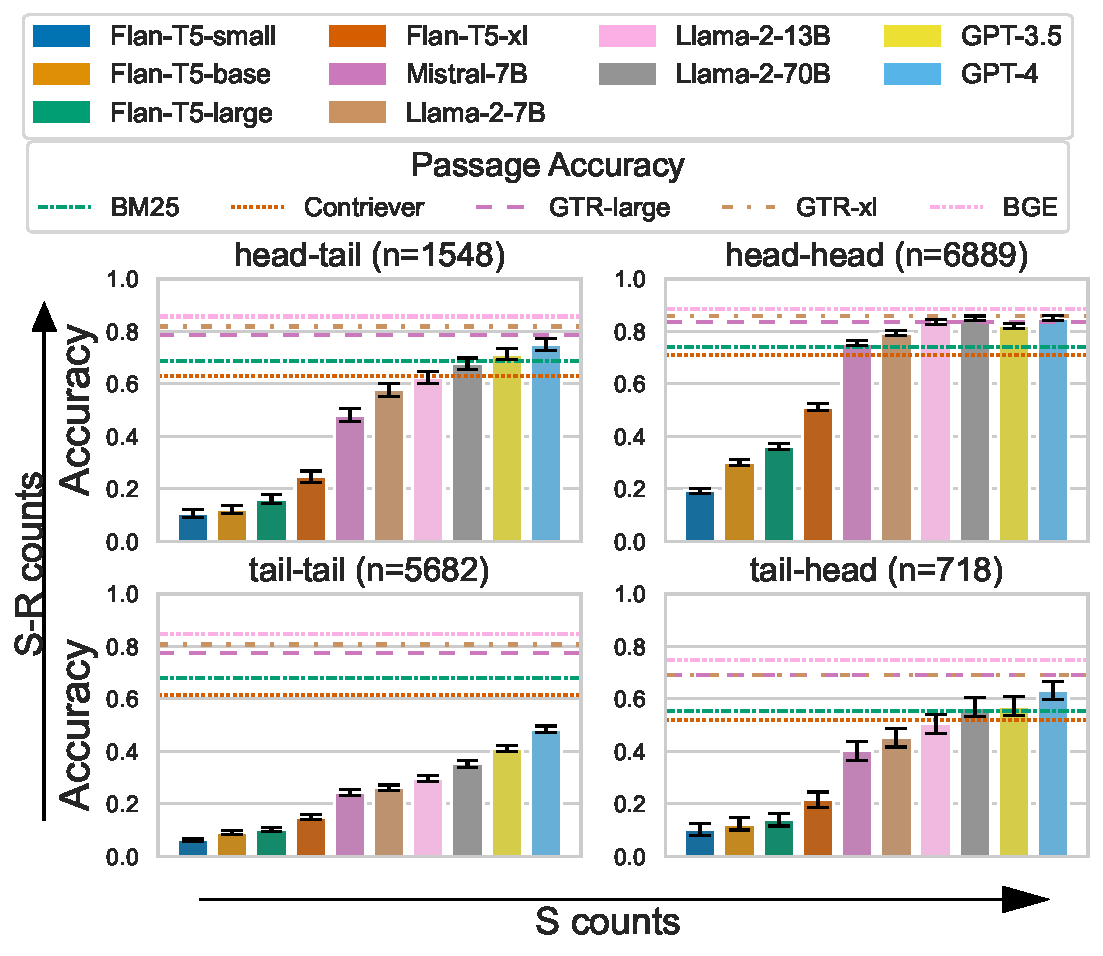
\includegraphics[width=0.48\textwidth]{submissions/Estevam2024/figures/head_tail_witqa200_for_vanilla_gtr.pdf}
    \caption{Analysis on Vanilla LMs with BM25, Contriver, GTR, and BGE passage accuracy over S-R counts and S counts ($n=$ the number of questions in the group). In the top row, S-R counts are higher than the median. In the bottom row, they are less than or equal to the median. In the left column, S counts are less than or equal to the median, and in the right column, they are higher than the median.} 
    \label{fg:head_tail_vanilla}
\end{figure}

\begin{itemize}
    \item LMs can often recall frequently encountered entity-relation pairs from pre-training without retrieval, but this depends on model size; larger models capture more long-tail relations for popular entities, though accuracy drops for less common facts.
    \item For long-tail entity-relation pairs, retrieval performs better than LM recall, suggesting retrieval augmentation benefits these cases but may introduce override issues with well-known pairs.
    \item LMs outperform retrievers on well-known entity-relation pairs involving long-tail entities, contrasting prior studies where large LMs struggled with these pairs.
\end{itemize}

\noindent
Using these insights, a selective memory integration module was designed, that applies retrieval augmentation or LM recall based on entity-relation popularity. The main idea is closely related to a System 2 approach, in which before trying to answer a question, the system first tries to figure out (reasoning task) whether it should use the retrieval mechanism or not.  It was found it could improve QA performance by up to 10.1\% \cite{maekawa-etal-2024-retrieval}.

%% Text Operators
Another limitation of most current RAG models is characterized by their reliance on localized context retrieval, making them less effective for tasks that require \textit{holistic reasoning}—the ability to synthesize, aggregate, and analyze information across multiple documents. For instance, when asked, ``Which company employed the most people?'' traditional retrieval models may return individual statistics for each company without a comprehensive comparison. This core limitation reveals that while RAG systems are adept at fact retrieval, they falter with broader, cross-document reasoning. Bridging this gap requires models capable of multi-document synthesis, comparative analysis, and extensive dataset integration.

One alternative to to address these limitations of RAG models in holistic reasoning is to bypass retrieval altogether and use long-context language models (LCLMs).  These models are designed to handle and process significantly larger chunks of information, enabling them to reason effectively over extensive contexts or large sets of documents without the need for iterative retrieval steps. By eliminating the dependency on retrieval mechanisms, LCLMs reduce the risk of retrieving irrelevant or incomplete information, which can compromise reasoning quality. Furthermore, their ability to maintain coherence across lengthy inputs makes them particularly well-suited for tasks requiring nuanced understanding, cross-referencing of details, and synthesis of insights from diverse sources within a single reasoning framework.

To investigate into this, \cite{maekawa2024holistic} conducted a comparative study of LCLMs and RAG models using HoloBench, a benchmark specifically designed to evaluate holistic reasoning capabilities. It compared two large LCLMs, Llama-3.1-405b and GPT-4o, alongside a smaller LCLM, Llama-3.1-8b. For document retrieval, the work employed \texttt{\small BAAI/bge-large-en-v1.5}, an effective embedding-based model that retrieves the 2k tokens most similar to the query.

The findings in \cite{maekawa2024holistic}  reveal that as context length exceeds 4k tokens, larger vanilla LCLMs consistently outperform RAG-based models, indicating their superior ability to manage longer contexts where RAGs struggle to retrieve relevant information (see Figure ~\ref{fig:rag}). Interestingly, with smaller models like Llama-3.1-8b, RAG performs better when context length surpasses 16k tokens. This aligns with previous findings\cite{maekawa-etal-2024-retrieval} that retrieval models can enhance the performance of weaker models by compensating for their reasoning limitations, even in the presence of retrieval errors. A promising future direction would be to adopt a System 2-based approach and integrate a dynamic mechanism for determining the optimal amount of information to retrieve based on the query and context length, particularly when working with weaker models for holistic reasoning.

\begin{figure}[ht]
    \centering
    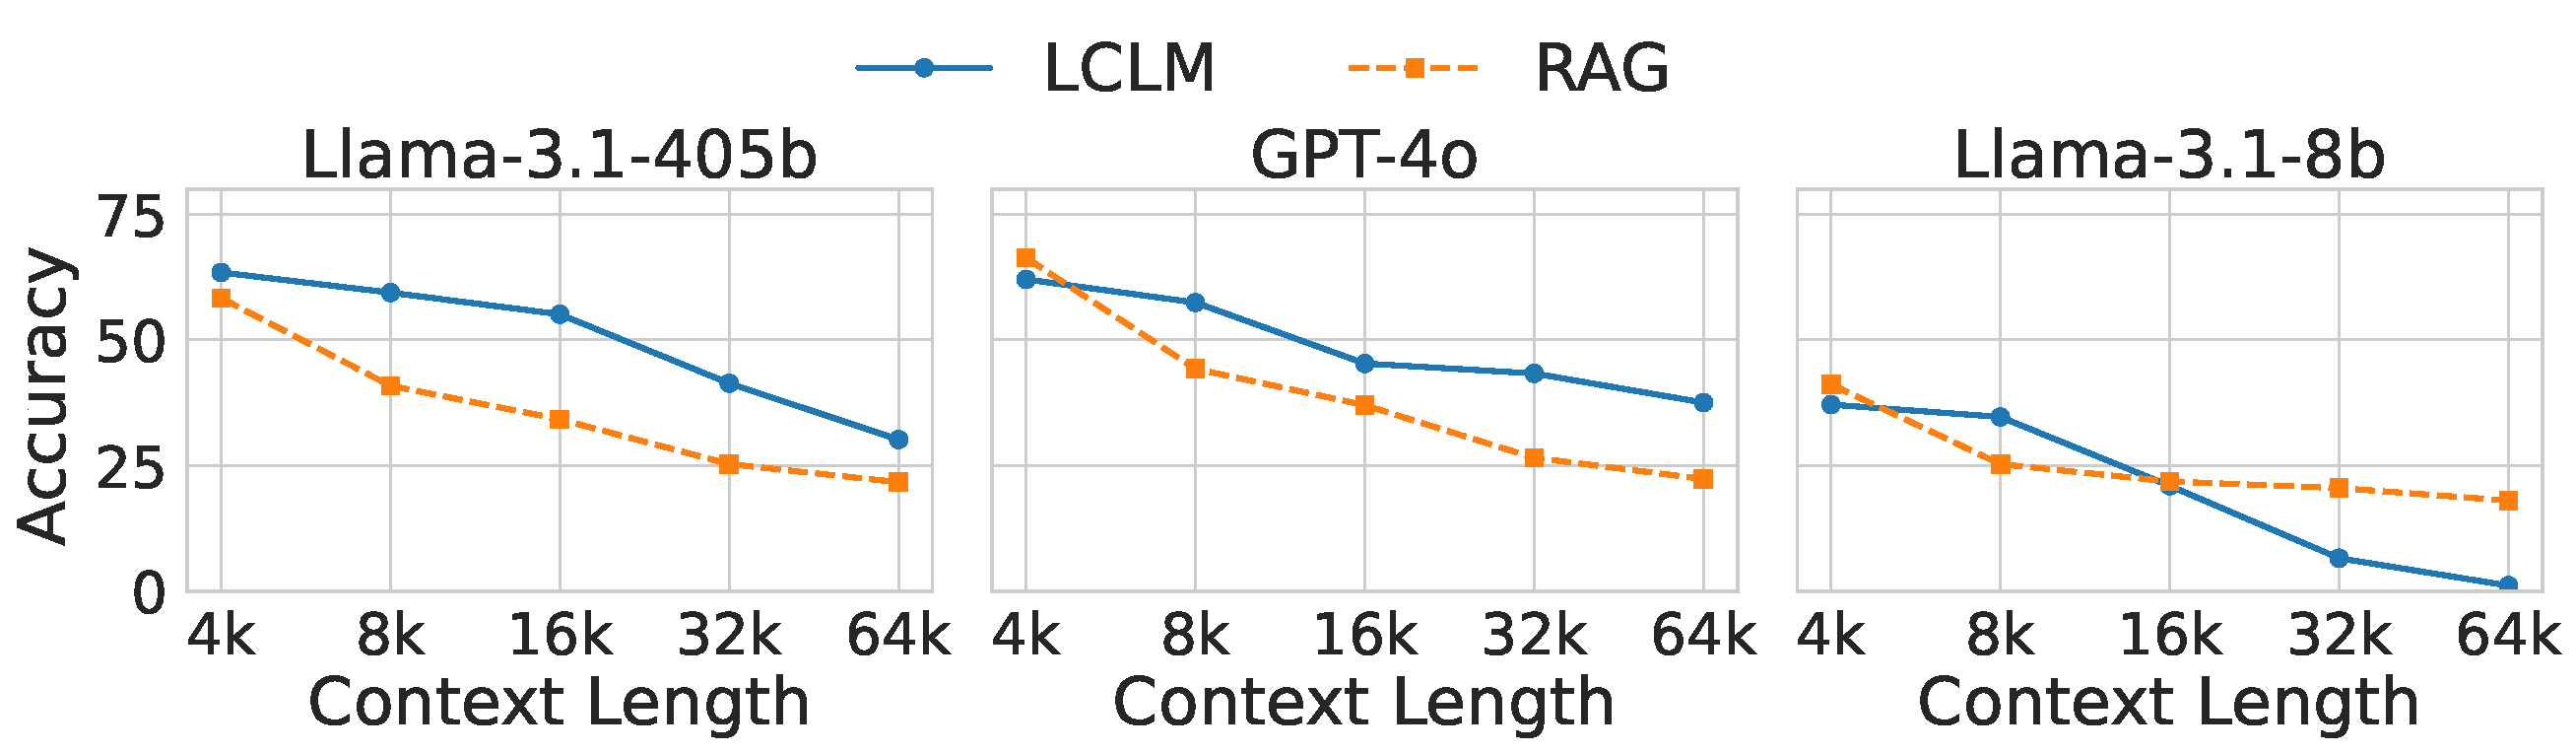
\includegraphics[width=.8\linewidth]{submissions/Estevam2024/figures/lclm_vs_rag_all_models.pdf}
    \caption{Performance comparison of LCLM and RAG. For long contexts, large models outperform RAG but a retriever helps a small model due to its limited ability to handle long contexts. }
    \label{fig:rag}
\end{figure}

\subsubsection{Impact of Prompt Sensitivity}

% \subsubsection{Revisiting LLM Reliability}
A notable limitation of LLMs is their sensitivity to the arrangement of components within prompts, which directly influences their performance in understanding and reasoning on specific tasks. Prior research has shown that LLMs are affected by the ordering of few-shot demonstrations \cite{zhao2021calibrate}. These findings raise an important question: are LLMs similarly affected by the order of elements in prompts across diverse tasks? For instance, in multiple-choice question (MCQ) answering tasks, does the order of answer options impact LLM performance? Figure \ref{fig:over} (extracted from \cite{pezeshkpour2024large}) shows the sensitivity of GPT-4 to options order using a sample from the common sense QA benchmark.  Within this context, \cite{pezeshkpour2024large} aims to address the following research questions: 
(1) To what extent do LLMs exhibit sensitivity to the order of options in multiple-choice questions? 
(2) What factors contribute to LLMs' sensitivity to the order of options? 

\begin{figure}[th!]
    \centering
    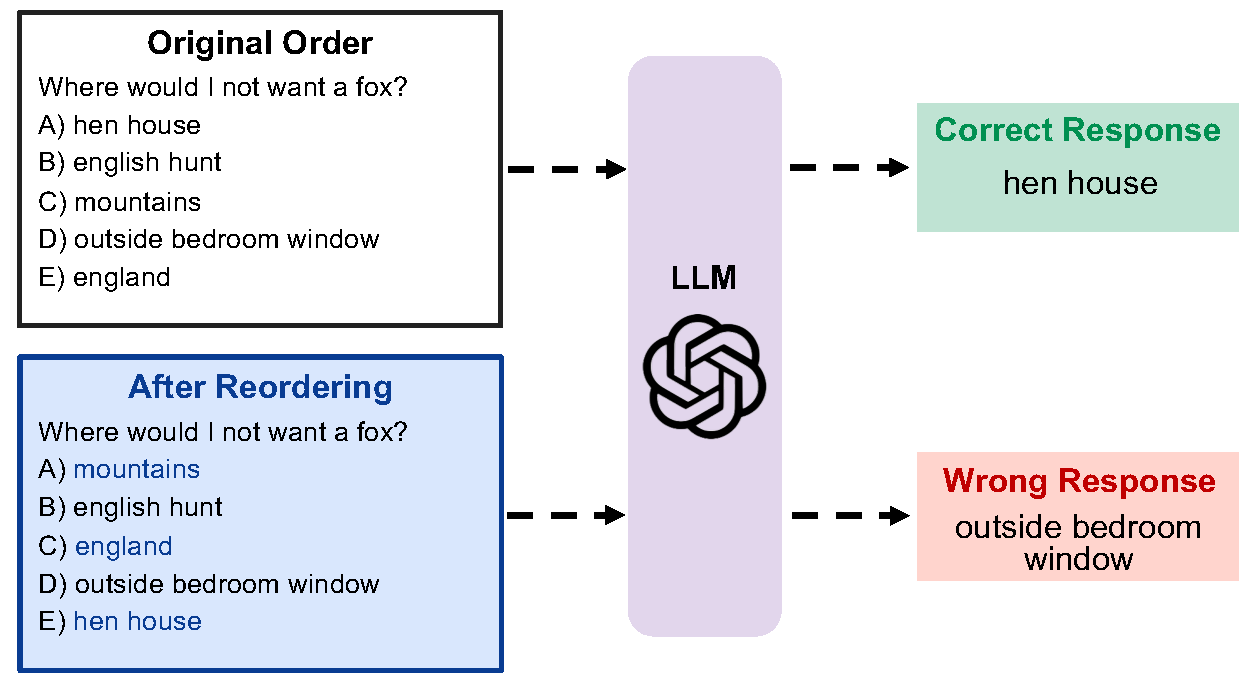
\includegraphics[width=0.7\columnwidth]{submissions/Estevam2024/figures/overview-mcq.pdf}
    \caption{{GPT-4 sensitivity to reordering options:} Upon changing the order of choices, GPT-4 changes its prediction from ``hen house'' to ``outside of bedroom window'' (the example is from the CSQA dataset).}
    \label{fig:over}
     % \minipostspace
\end{figure}

To address the first question, \cite{pezeshkpour2024large} conducted experiments using GPT-4, InstructGPT (text-davinci-003), and Llama-2-13b (chat version) across five multiple-choice question benchmarks. A surprisingly high sensitivity gap of up to 85\% in the zero-shot setting (see Table ~\ref{tab:attack-zero}) was found. Furthermore, in the few-shot setting, introducing demonstrations to the prompt led only to marginal gains in robustness, if any improvement was observed.

\begin{table*}[th!]
\small
\centering
\begin{tabular}{lrrrrrrrrr}
\toprule 
\multirow{2}{*}{\bf Tasks} & \multicolumn{3}{c}{\bf GPT-4}&  \multicolumn{3}{c}{\bf InstructGPT}&  \multicolumn{3}{c}{\bf Llama-2-13b}\\
\cmidrule(lr){2-4}
\cmidrule(lr){5-7}
\cmidrule(lr){8-10}
&Vanila&Min&Max&Vanila&Min&Max&Vanila&Min&Max\\
\midrule
CSQA &84.3&\color{cadmiumred}{-12.6}&\color{cadmiumgreen}{+10.3}&72.3&\color{cadmiumred}{-24.0}&\color{cadmiumgreen}{+19.1}&62.2&\color{cadmiumred}{-28.9}&\color{cadmiumgreen}{+25.5}\\
Logical Deduction&92.3&\color{cadmiumred}{-8.1}&\color{cadmiumgreen}{+5.0}&64.0&\color{cadmiumred}{-39.4}&\color{cadmiumgreen}{+34.7}&53.0&\color{cadmiumred}{-30.7}&\color{cadmiumgreen}{+34.7}\\
Abstract Algebra &57.0&\color{cadmiumred}{-30.0}&\color{cadmiumgreen}{+23.0}&33.0&\color{cadmiumred}{-31.0}&\color{cadmiumgreen}{+39.0}&32.0&\color{cadmiumred}{-32.0}&\color{cadmiumgreen}{+53.0}\\
High School Chemistry &71.9&\color{cadmiumred}{-23.6}&\color{cadmiumgreen}{+18.2}&44.8&\color{cadmiumred}{-28.5}&\color{cadmiumgreen}{+38.0}&40.6&\color{cadmiumred}{-32.7}&\color{cadmiumgreen}{+45.6}\\
Professional Law &66.1&\color{cadmiumred}{-12.7}&\color{cadmiumgreen}{+12.1}&48.6&\color{cadmiumred}{-24.9}&\color{cadmiumgreen}{+25.7}&43.8&\color{cadmiumred}{-32.8}&\color{cadmiumgreen}{+32.9}\\
\bottomrule
\end{tabular}
\caption{\textbf{Zero-shot order sensitivity}; all three LLMs display a notable level of sensitivity to the order of options across various benchmarks.}
\label{tab:attack-zero}
\end{table*}

\begin{figure*}[th!]
    \centering
    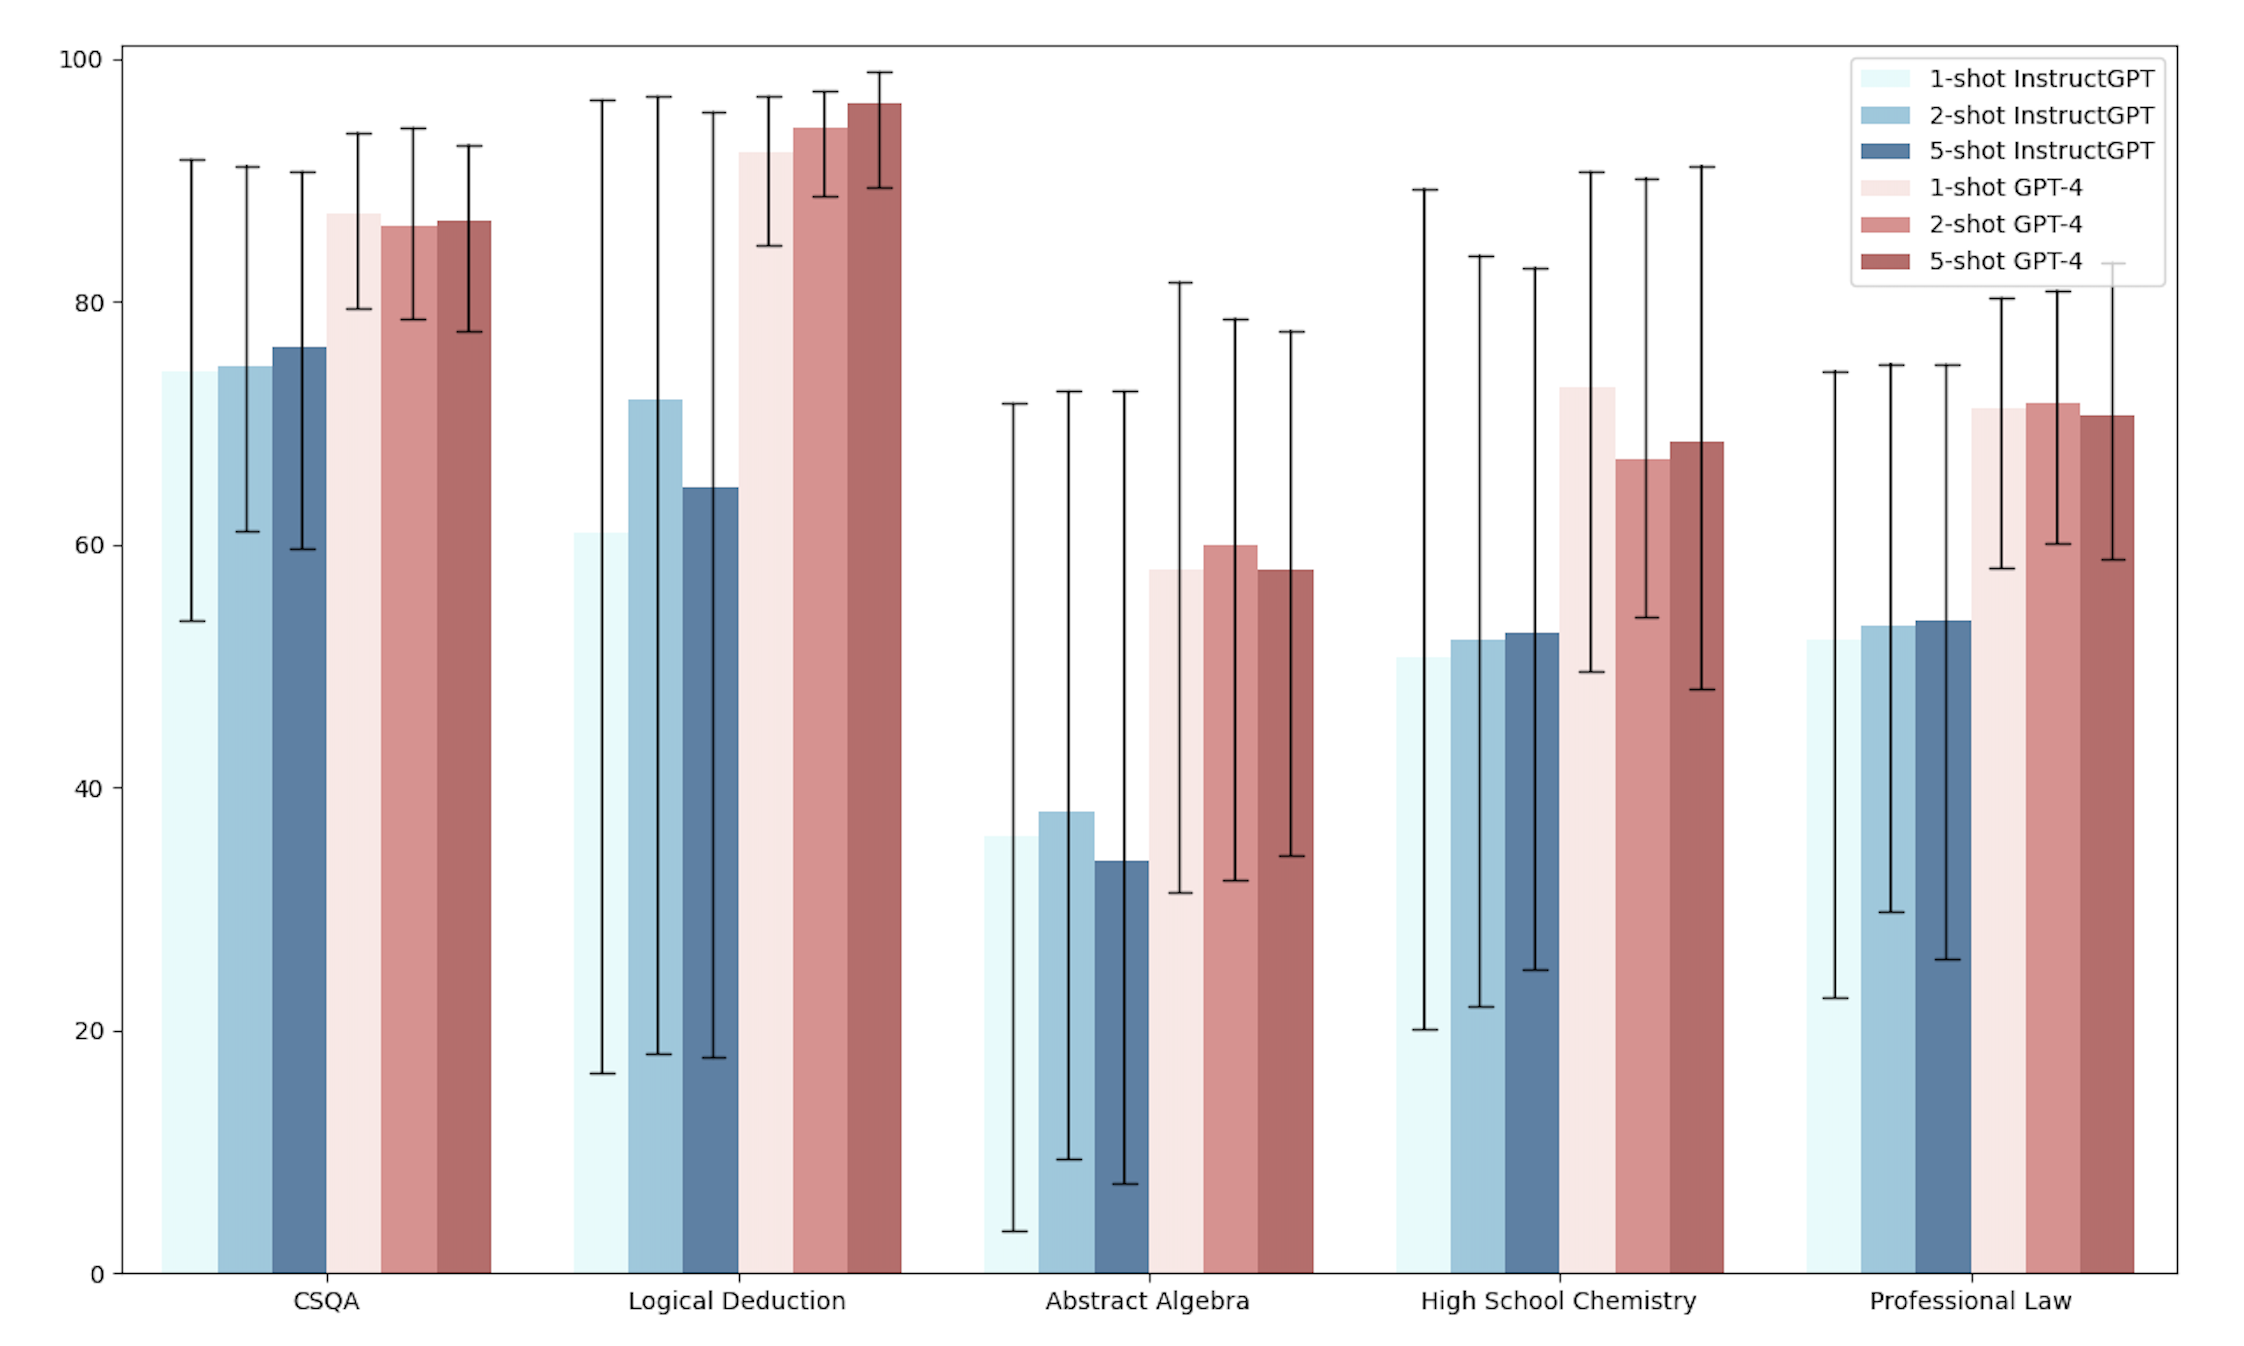
\includegraphics[width=0.5\paperwidth]{submissions/Estevam2024/figures/few-shot-order.png}
    \caption{\textbf{Order sensitivity in the few-shot setting:} The error bars represent the range of minimum and maximum accuracy achievable in each task through oracle reordering. Our observations are as follows: (1) The sensitivity gap consistently remains substantial in the few-shot setting. (2) As performances improve, the sensitivity gap shrinks. (3) Adding more demonstrations does not necessarily results in a reduction of the gap.}
    \label{fig:few-sens}
\end{figure*}

Regarding the second question, it is hypothesized that this sensitivity arises from positional bias, where LLMs display a preference for certain answer placements when uncertain. To investigate, \cite{pezeshkpour2024large} analyzed instances where the models’ predictions shifted upon reordering answer options. Additionally, was also found that increasing the number of options, while keeping the top possible answers, only gradually affected performance, suggesting that positional bias rather than option count plays a larger role in LLM sensitivity (see Figure ~\ref{fig:few-sens}). 

Another interesting finding from \cite{pezeshkpour2024large} is that, instead of using the original order of the multiple-choice options, one can adopt a "system 2" approach and reason before output the first answer generated by the LLM. In this sense, before deciding on the final answer for the question, the same question can be posed to the LLM multiple times (five times in the referenced study), each time with a randomly shuffled set of choices. Afterward, the answers are aggregated through a reasoning mechanism (in the paper, a very simple majority voting reasoning was employed). This approach has been shown to improve the LLM's overall performance.  






%todo
% \subsubsection{Reliable Decision Making w/ RAG}
\subsubsection{Transparency and Accountability in Downstream Applications}
\label{sec:rag_accountable}
To study the implications of trust and accountability of RAG pipelines in downstream applications, \cite{mishra2023characterizing} considers the task of generating natural language explanations of knowledge-intensive task (KIT) decisions such as multiple-choice question answering. Given the setting for generating corroborating and refutation complete rationales for KIT model decisions, the suitability of retrieval-augmented rationale generation using LLMs is explored. The prompt to LLMs is enriched with relevant knowledge from external sources to condition the rationale generation on facts. Three human subject studies were conducted to evaluate the effectiveness of such rationales in communicating KIT model decisions. 

More specifically, two studies were conducted, via crowdsourcing, to evaluate the preferability and acceptability of such rationales to crowd-workers. In another study involving experts --- motivated by existing literature on trust in explainable AI~\cite{hoffman2018metrics, stites2021sage} --- the implications of faithfully rationalizing KIT model decisions irrespective of their correctness was explored.
The crowd-sourced studies demonstrate that, more often than not, crowd workers prefer LLM-generated
rationales to crowdsourced rationales in existing datasets, citing their factuality, sufficiency, and convincing refutation. 
Follow-up fine-grained analysis 
reveals that LLM-generated rationales
still have significant room for improvement along
dimensions such as \emph{insightfulness} (\ie providing new information), \emph{redundancy} (\ie avoiding repetitive text), and \emph{generalizability} (\ie domain invariance.)
The expert-sourced study confirms that faithful rationalization of incorrect model predictions 
degrades humans' trust in the generated rationales. 
The work further explores the utility of instrumenting mechanisms
to intervene in the incorrect predictions via a review-then-rationalize pipeline instead of faithfully rationalizing and find that even simple strategies may help intervene up to $71\%$ of the incorrect predictions.

\begin{figure} 
\vspace{-10pt}
    \centering
    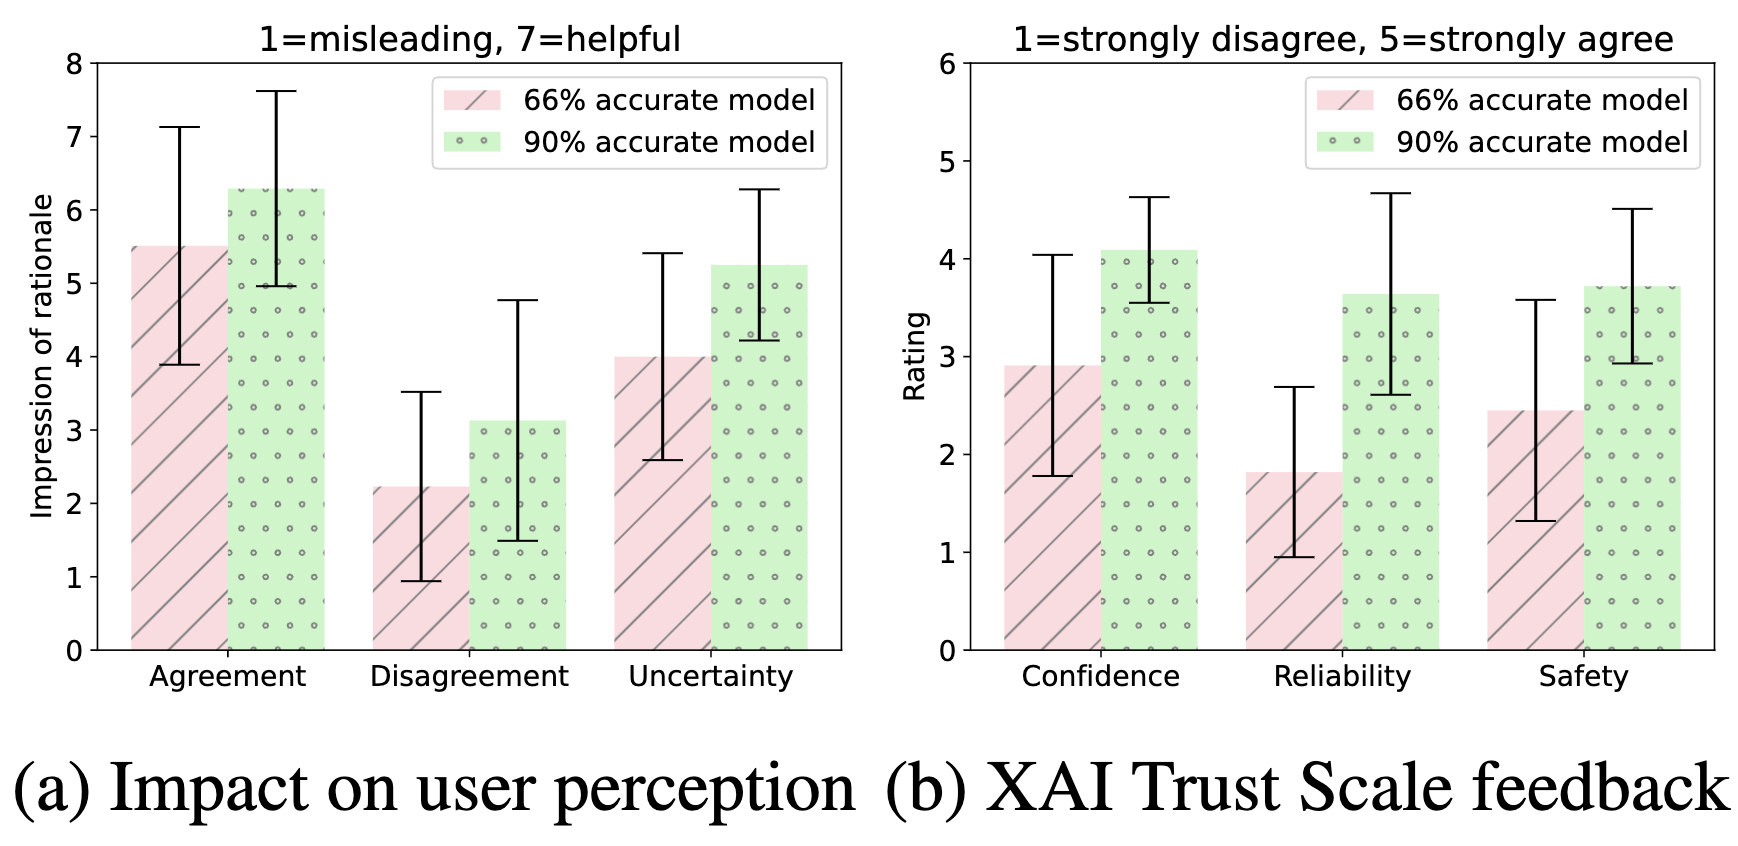
\includegraphics[width=0.6\linewidth]{submissions/Estevam2024/figures/xai-trust.png}
 
  \caption{(a) Irrespective of agreement or disagreement with the KIT model prediction, participants indicated a more negative impression about the rationalization of the lower confidence model prediction. (b) Participant feedback on the trust scale indicates lower confidence for lower accuracy model rationalization.}
  \label{fig:xai_rationale} 

\end{figure}

Figure~\ref{fig:xai_rationale}a \cite{mishra2023characterizing} summarizes the participants' impression of a rationale immediately after viewing the model prediction. When the participants disagreed with the model prediction, they exhibited a stronger negative impression about the rationales for the $66\%$ accuracy condition compared to the $90\%$ accuracy condition. Even when participants agreed with the model prediction, their impression of the rationales remained more negative. The intuition is that the higher disagreement with the model coupled with observing the faithful rationalization of the incorrect prediction negatively impacted participants' perception of the reliability of the rationales. These observations are confirmed by analyzing the results of the follow-up survey (see Figure~\ref{fig:xai_rationale}b.)  Unsurprisingly, participants for the $66\%$ accuracy condition rated their confidence in the generated rationales and the reliability of the rationalizer significantly lower compared to the $90\%$ accuracy condition.


